\chapter{Requirement}

The aim of the thesis is build a pervasive real-time system for smart-city, where we want use the AC paradigm over a LoRaWan network.

\section{Case study}

The system should use real-time data to create a city map of quality air.
The application will use the map to define a route to a destination that avoid areas with poor air quality.
Data can be produced by two types of sensors:
\begin{itemize}
    \item \textbf{Fixed}: positioned along the roads and at intersections
    \item \textbf{Mobile}: placed on public transport or bicycles
\end{itemize}

Sensors will use DingNet network to communicate their sensed data. DingNet is a network LoRa-over-MQTT where every device send data to all the gateways inside the communication range. Then the gateways publish sensors data on MQTT server for the application, \autoref{fig:LoRa}.

\begin{figure}[h]
    \centering
    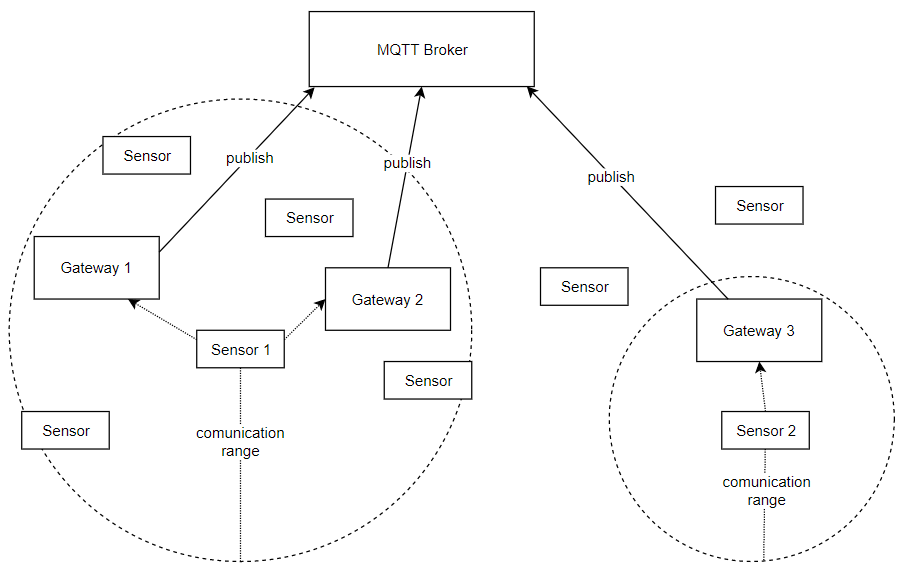
\includegraphics[scale=0.70]{LoRa.png}
    \caption{LoRa architecture}
    \label{fig:LoRa}
\end{figure}